\chapter[Results]{Results} \label{ch:results}

% Here we present the results of our primary and alternative optimization strategies.
Here we present the results of our optimization strategy.
Before reporting on the performance of our strategy, we first conduct preliminary analyses to refine our method.
% After finalizing these refinements, we report on the performance of this strategy.
All random circuits are generated using the \codeword{CNOT_HAD_PHASE_circuit} method in PyZX which constructs a circuit consisting of CNOT, HAD, and phase gates.
Default parameters are used for the probability of each gate type.


% \section{Primary Strategy}

\section{Refinements}

General opportunities for refinement are the following:
\begin{itemize}
\item
  Optimization function
\item
  Probability of applying Equation \ref{eq:gen-io-lc} vs. Equation \ref{eq:gen-io-pivot}
\item
  Sampling of subjects (i.e., spiders or pairs of connected spiders) for congruence application
% \item
  % Probability of applying \codeword{full_reduce} throughout search, $p_{fr}$ % FIXME: Could just skip this one...
\end{itemize}
For these analyses, we only use SA as it is more computationally efficient and we expect the behavior of these refinements to generalize to GA.

We also conduct procedure-specific refinements.
We analyze how varying the number of iterations or mutants and generations affects optimization using SA and GA, respectively.

\subsection*{Optimization Function}

First, we test if any property of a ZX-diagram could serve as a reliable proxy for the complexity of its associated circuit.
To do so, we first generated 500 random circuits (10 qubits, 100 gates) and immediately converted them to ZX-diagrams.
Given this library of ZX-diagrams, we then measured the Pearson correlation coefficient between the complexity of the extracted circuit and each ZX-diagrammatic property discussed in Section \ref{sec:obj-funcs}.
The following table summarizes these correlations:
\begin{center}
  % \begin{table*}[h!]
  % \begin{tabular}[]{@{}lcc@{}}
\begin{tabular}[]{@{}l>{\centering\arraybackslash}p{1.5cm}>{\centering\arraybackslash}p{2cm}@{}}
\toprule
                    & $r$ & p-value \\ \midrule
\# Edges  & 0.097        & 0.029            \\
Centrality & 0.090        & 0.045            \\
Density    & -0.096       & 0.032            \\ \bottomrule
\end{tabular}
% \caption{\label{tab:obj-pearson}Correlations between various ZX-diagrammatic properties and the complexity of the extracted circuit for 500 randomly generated ZX-diagrams. Pearson's correlation coefficient is denoted $r$ and the 2-tailed p-value is provided. The ZX-diagrams were generated by converting 500 random circuits with 10 qubits and 100 gates to ZX-diagrams.}
% Table \ref{tab:obj-pearson} summarizes these correlations.
% \end{table*}
\end{center}
Pearson's correlation coefficient is denoted $r$ and the 2-tailed p-value is provided.
From these data, it is clear that no identified property of a ZX-diagram can serve as a reliable proxy for the complexity of its associated circuit.
Therefore, the default scoring method discussed in Section \ref{sec:strategy} that relies on extraction is used for the remainder of our analyses.



\begin{figure}[t]
\centering
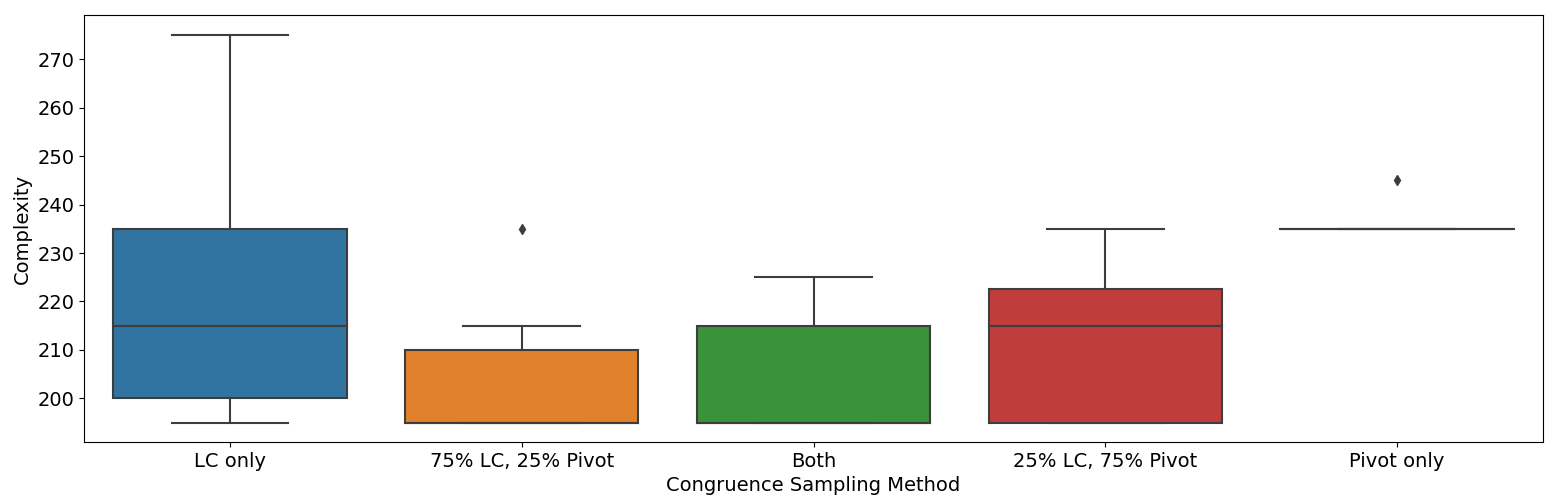
\includegraphics[width=13cm]{img/cong-sampling-ex.png}
\caption{
  A representative comparison of congruence sampling methods for a 5 qubit, 50 gate circuit.
  All three sampling methods that include both LC and pivoting achieve the best simplification in the alotted number of steps.
  When using only local complementation (i.e., Equation \ref{eq:gen-io-lc}), the same best-case complexity is achieved over the 10 trials but the average complexity is higher.
  Alternatively, using only pivoting does not achieve the same reduced circuit.
}
\label{fig:cong-sampling}
\end{figure}

\subsection*{Congruence Sampling}

By default, we apply Equations \ref{eq:gen-io-lc} and \ref{eq:gen-io-pivot} with equal probability ($p_{LC} = p_{pivot} = 0.5$).
However, it may be the case that one congruence should be chosen more frequently than the other.
To evaluate this, we generated 30 random circuits (5 qubits, 50 gates) and repeated search with a range of $(p_{LC}, p_{pivot})$ pairs.
For a given circuit, search was performed 10 times for each pair and the complexities of the optimized circuits were plotted according to congruence sampling probabilities.
In all cases, the sampling methods that include both LC and pivoting yielded the lowest average complexity across the 10 trials as well as the least complex circuit overall.
% In some cases, other sampling methods matched, but never outperformed this method in either metric.
There were no significant differences between the three combined sampling methods (i.e., 50/50, 25/75, and 75/25) and the LC- ($p_{LC} = 1.0$, $p_{pivot} = 0.0$) or pivot-only ($p_{LC} = 0.0$, $p_{pivot} = 1.0$) sampling methods sometimes matched, but never outperformed these combined methods.
% Most notably, the least cusing only local complementation (i.e., $p_{LC} = 1.0$, $p_{pivot} = 0.0$) produced a circuit that matched the
Most notably, the least complex circuit identified using LC-only matched the minimum complexity 73.3\% of the time while that identified using pivot-only was more complex than the best-case 86.7\% of the time.
% Most notably, the least complex circuit identified using only local complementation (i.e., $p_{LC} = 1.0$, $p_{pivot} = 0.0$) matched the minimum complexity found via 50/50 sampling FIXME\% of the time and was less complex than that found using only pivoting FIXME\% of the time (and otherwise no more complex).
% Most notably, the minimum-complexity circuit identified using LC-only (i.e., $p_{LC} = 1.0$, $p_{pivot} = 0.0$) matched that found via 50/50 sampling
% method most commonly matched the default and almost always outperformed the pivot-only method.
% LC-only (i.e., $p_{LC} = 1.0$, $p_{pivot} = 0.0$) and
A representative comparison for one random circuit is shown in Figure \ref{fig:cong-sampling}.

The observation that LC-only typically outperforms pivot-only is intuitive as one pivot is equivalent to three local complementations and therefore LC-only enables a more fine-grained search.
While LC-only likely converges to the combined sampling methods in the limit, we retain pivoting in the action set as it appears to require a fewer number of iterations at no cost.
% However, since LC-only always matches and never outperforms the equal sampling of either congruences,
In the remainder of our analyses, the default uniform sampling of Equations \ref{eq:gen-io-lc} and \ref{eq:gen-io-pivot} (i.e., $p_{LC} = p_{pivot} = 0.5$) is used.


\begin{figure}[t]
\centering
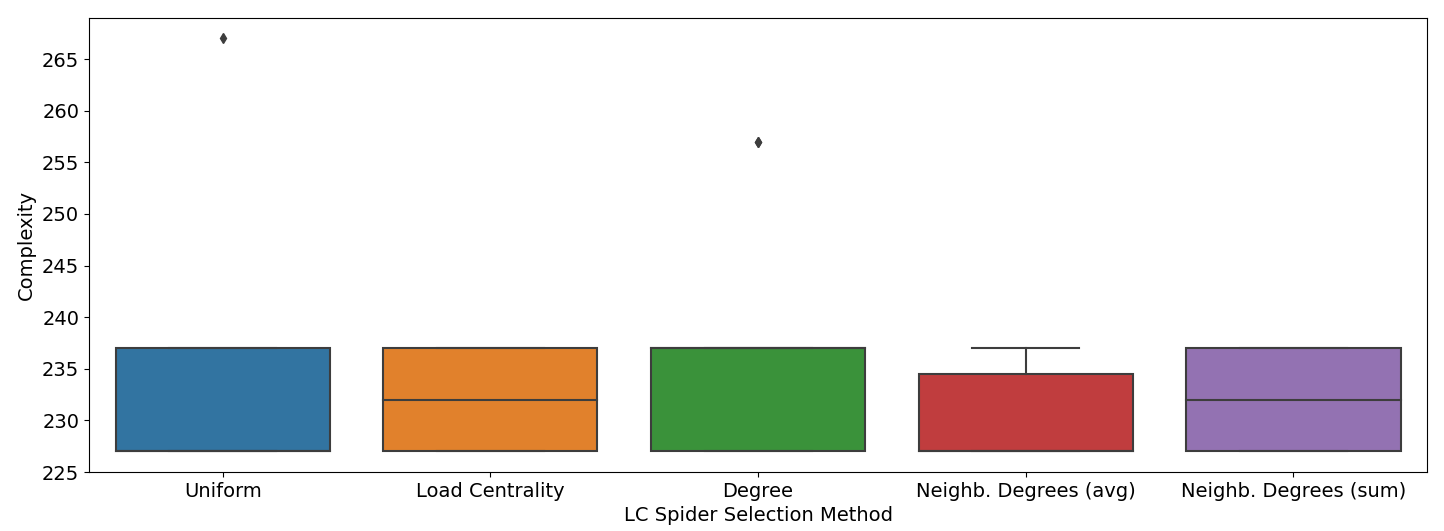
\includegraphics[width=13cm]{img/subj-sampling-ex.png}
\caption{
  A representative example of optimization of a 5 qubit, 50 gate circuit with different metrics of sampling spiders for application of Equation \ref{eq:gen-io-lc}.
  Optimization was performed 10 times for each sampling method using SA.
  No significant differences are observed in performance across the different weightings.
}
\label{fig:subj-sampling}
\end{figure}


\subsection*{Congruence Subject Sampling}

Similar to the probabilistic sampling of congruences to apply throughout search, we can experiment with methods of sampling subjects (i.e., spiders or pairs of connected spiders) for congruence application.
By default, we sample from the set of all eligible subjects uniformly.
However, we could alternatively weight this sampling in a way that improves search.
Candidate metrics for Equations \ref{eq:gen-io-lc} and \ref{eq:gen-io-pivot} are discussed in Section \ref{sec:strategy}.

To test these alternative weightings, we employ a similar approach as for congruence sampling.
First, we restrict the action space to that congruence for which we are testing various weightings to isolate its effect.
For example, if we are testing various weighting metrics to select a spider for application of Equation \ref{eq:gen-io-lc}, we set $p_{LC} = 1.0$ and $p_{pivot} = 0.0$.
We then proceed as before, evaluating the performance of SA on random circuits across 10 trials for each candidate weighting.
We evaluate 20 random circuits (5 qubits, 50 gates) for each set of sampling procedures.

In both cases, no sampling method demonstrated reliable improvement over any other across the 20 trials.
One representative example of this comparison for sampling spiders for Equation \ref{eq:gen-io-lc} is shown in Figure \ref{fig:subj-sampling}.
Similar results were observed for sampling pairs of connected spiders for Equation \ref{eq:gen-io-pivot}.
So, for the remainder of our analyses, we sample subjects for congruence application uniformly.

\begin{figure}[t]
\centering
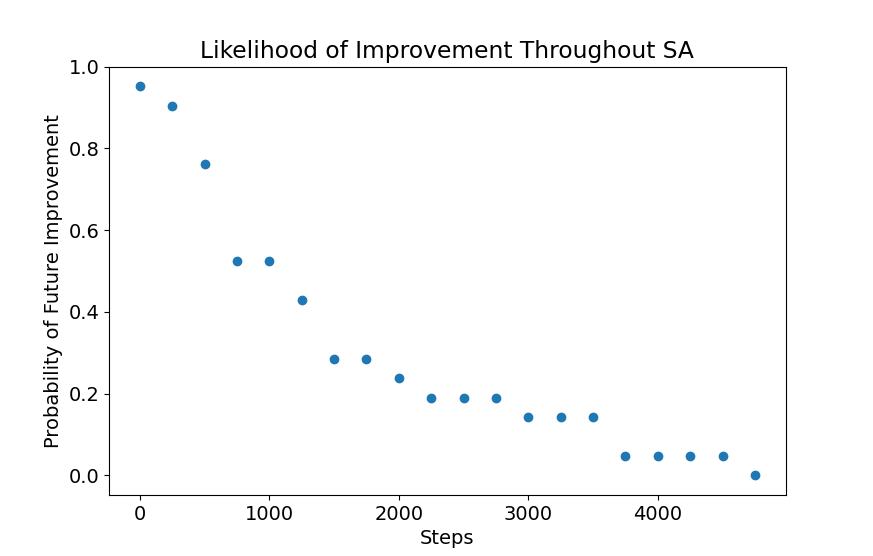
\includegraphics[width=13cm]{img/iter-likelihood.png}
\caption{
  The likelihood of obtaining a ZX-diagram with a simpler extracted circuit after a given iteration in SA.
  For example, after 2000 steps, there is a 20\% chance of obtaining a ZX-diagram corresponding to an even simpler circuit as search progresses.
  These data were obtained using circuits with 4-10 qubits and 10-20 gates per qubit and do not necessarily generalize to larger circuits.
}
\label{fig:iter-likelihood}
\end{figure}

\subsection*{Number of SA Iterations}

The maximum number of SA steps $k_{max}$ should be high enough to permit the bulk of optimization while low enough to be computational feasible.
We determine the optimal $k_{max}$ by optimizing a set of random circuits and computing the probability that SA uncovers a complexity reduction after fixed intervals.
First, we generated a set of 36 random circuits with 4-10 qubits (intervals of 2) and 10-20 gates per qubit (intervals of 5).
For each circuit, we obtained a simplified ZX-diagram via \codeword{teleport_reduce} + \codeword{basic_optimization}.
We then optimized each simplified ZX-diagram using SA with $k_{max} = 5000$ and recorded the complexity of the best circuit every 250 steps.
Lastly, we computed the probability that a ZX-diagram whose extracted circuit is less complex would be found as search progressed for each 250-step interval.
% Lastly, we computed the probability that a less-complex circuit would be found as search progressed for each 250-step interval.
% We repeated this entire analysis twice, once for each method of obtaining a simplified ZX-diagram from a circuit (see Figure \ref{fig:primary}).

The results of this analysis are shown in Figure \ref{fig:iter-likelihood}.
We see that most improvement occurs in the beginning of search and that the chance of finding a simpler circuit after 2500 steps is less than 10\%.
For this reason, we fix $k_{max} = 2500$ for the remainder of our analyses unless otherwise noted.


\begin{figure}
\centering
\begin{subfigure}[t]{0.47\textwidth}
  \centering
  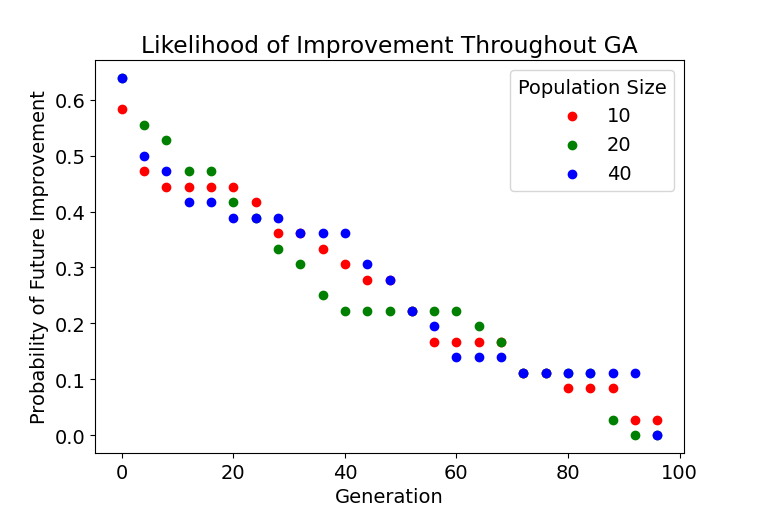
\includegraphics[width=\linewidth]{img/ga-likelihood.png}
  \caption{The likelihood of obtaining a simpler circuit after a given generation.
  As in Figure \ref{fig:iter-likelihood}, these data were obtained using circuits with 4-10 qubits and 10-20 gates per qubit.}
  \label{fig:ga-likelihood}
\end{subfigure}
\hfill
\begin{subfigure}[t]{0.47\textwidth}
  \centering
  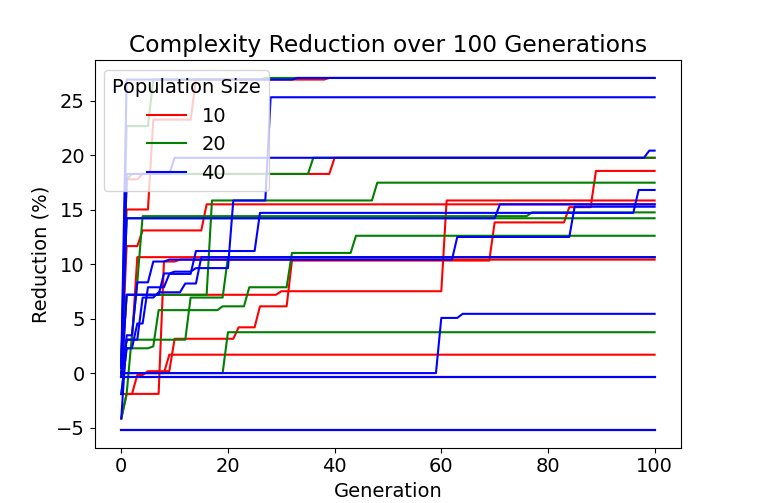
\includegraphics[width=\linewidth]{img/7qb}
  \caption{
    The reduction in complexities over time for 10 random 7 qubit, 100 gate circuits.
    Reduction in complexity is measured with respect to the simplified ZX-diagram rather than the original circuit.
  }
  \label{fig:7qb}
\end{subfigure}
\caption{
  GA parameter tuning
}
\label{fig:ga-params}
\end{figure}


\iffalse
\begin{figure}[t]
\centering
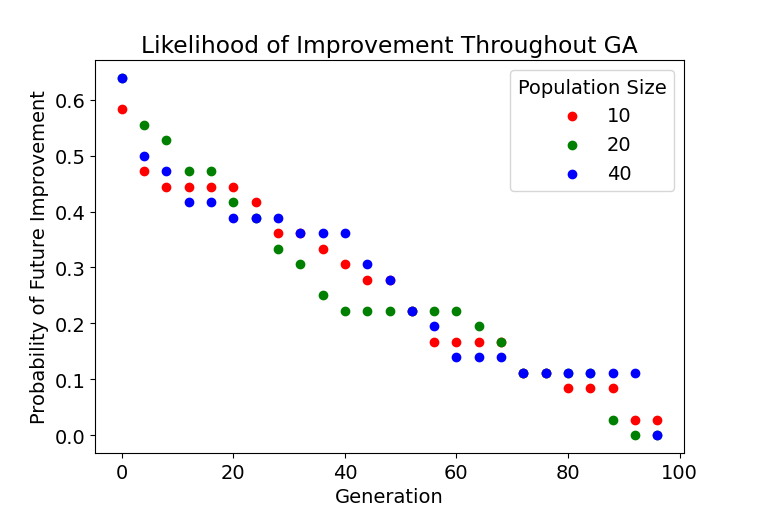
\includegraphics[width=13cm]{img/ga-likelihood.png}
\caption{
  The likelihood of obtaining a ZX-diagram corresponding to a simpler circuit after a given generation in GA.
  As in Figure \ref{fig:iter-likelihood}, these data were obtained using circuits with 4-10 qubits and 10-20 gates per qubit.
}
\label{fig:ga-likelihood}
\end{figure}
\fi


\subsection*{GA Parameters}

Similarly, when searching this space with GA, we want to evolve a large enough population for sufficiently many generations while incurring minimal computational cost.
To determine the appropriate population size and number of generations, we employ a similar approach as for determining $k_{max}$.
First, we generated a set of 36 simplified ZX-diagrams in the same fashion.
We then evolved each ZX-diagram for 100 generations with a population of 10, 20, or 40 mutants.
Lastly, for each population size, we computed the probability that a ZX-diagram corresponding to a simpler circuit (via extraction) would be found as search progressed for each 2-generation interval.
These probabilities for each population size are shown in Figure \ref{fig:ga-likelihood}.
Interestingly, all three population sizes exhibit similar behavior.
% Additionally, almost 50\% of all evolutions either perform all optimization in the 0th generation or provide no improvement.

We also sought to understand both the rate of reduction (with respect to the simplified ZX-diagram) over time and differences in total reduction between population sizes.
We plotted the complexity reduction over time for 10 random circuits with 7 qubits and 100 gates for each population size.
% We also generated 10 random circuits with 7 qubits and 100 gates and plotted the complexity reduction
% We also plot the complexity reduction (with respect to the simplified ZX-diagram) over time for each circuit both to evaluate the rate of reduction and to identify differences in total reduction between population sizes.
These reductions (one line per circuit for each population size) are shown in Figure \ref{fig:7qb}.
% note that there is particularly high variance in performance as the circuits have a variable number of qubits.
It is immediately clear that most optimization occurs in the first few generations.
Additionally, there is no reliable benefit provided by a larger population size.
We fix $n_{mutants} = 20$ and $n_{gens} = 40$ for the remainder of our analyses unless otherwise stated.

\section{Performance}

After refining the parameters of our method, we seek to understand our method's overall capabilities.

\subsection*{Further Simplification of ZX-Diagrams}

First, we want to understand our procedure's ability to further optimize a simplified ZX-diagram.
In this sense, we are not (yet) comparing the two methods of obtaining this initial ZX-diagram and complexity reduction is measured with respect to the simplified ZX-diagram that seeds search.
We test this by optimizing the simplified ZX-diagrams of 10 randomly generated circuits for $4, 6, \dots 14$ qubits with either 10 or 25 gates per qubit.
% First: Reduction capabilities for either TR or FR input. Not comparing TR vs. FR. Show for both SA and GA. This is telling us performance with respect to qubits, and also SA vs GA.
% First, we test the performance of our procedure for varying circuit sizes.
% Given a simplified ZX-diagram, we are initially only interested in our procedure's ability to further optimize the corresponding circuit;
% % Importantly, we are initially only interested in the reduction in complexity from the circuit associated with the simplified ZX-diagram rather than the original circuit.
% in this sense, we are not (yet) comparing the two methods of obtaining this initial ZX-diagram.
% For $4, 6, \dots 14$ qubits, we optimize the simplified ZX-diagrams of 10 randomly generated circuits with either 10 or 25 gates per qubit.
% We then plot the average reduction with respect to the simplified ZX-diagram.
We repeat this analysis for all four combinations of the two search procedures and the two ZX-diagram simplification methods.

Figure FIXME contains plots of average reductions for all four combinations.
% FIXME: analysis. most likely can always provide benefit, and SA and GA are similar. cant for higher qubits, and might make more progress on the FR one.


% \subsection*{Comparison of Search Procedures and Initial Simplifications}
\subsection*{Improving Optimization of the Original Circuit}

% Okay, we know we can improve on the simplified ZX-diagram. Now, want to compare for performance on input circuit.
After demonstrating that our method can further simplify ZX-diagrams for circuits with a sufficiently low number of qubits, we want to understand how these graph-level simplifications translate to optimization of the original circuit.

% Then, if we are concerned with optimizing the input circuit, is it better to apply congruences over FR or TR + basic simplified ZX-diagram? Compute some averages, and show a representative histogram with vertical lines.

% Then, took benchmarks from previous paper below qubit threshold. Did better.

\subsection*{Scaling Efforts}

% Then, we see if we can get higher qubits. Increase iterations, etc.

Lorem ipsum. I said lorem ipsum.

\begin{table}[]
\begin{tabular}{@{}ccccccc@{}}
\toprule
\multirow{3}{*}{\textbf{Qubits}}           & \multicolumn{6}{c}{\textbf{Complexity Reduction (\%)}}                                                      \\ \cmidrule(l){2-7}
                                           & \multirow{2}{*}{TR} & \multirow{2}{*}{FR} & \multicolumn{2}{c}{SA} & \multicolumn{2}{c}{GA} \\ \cmidrule(l){4-7}
                                           &                     &                     & TR seed    & FR seed   & TR seed    & FR seed   \\ \midrule
4                                          & 10                  & 10                  & 10         & 10        & 10         & 10        \\
6                                          & 10                  & 10                  & 10         & 10        & 10         & 10        \\
8                                          & 10                  & 10                  & 10         & 10        & 10         & 10        \\
10                                         & 10                  & 10                  & 10         & 10        & 10         & 10        \\
12                                         & 10                  & 10                  & 10         & 10        & 10         & 10        \\
14                                         & 10                  & 10                  & 10         & 10        & 10         & 10        \\ \midrule
\multicolumn{1}{l}{\textbf{Avg. Time (s)}} & 1                   & 1                   & 100        & 100       & 100        & 100       \\ \bottomrule
\end{tabular}
\end{table}
